\documentclass[a4paper,11pt,UTF8]{article}
\usepackage{ctex}
\usepackage{amsmath,amsthm,amssymb,amsfonts}
\usepackage{amsmath}
\usepackage[a4paper]{geometry}
\usepackage{graphicx}
\usepackage{microtype}
\usepackage{siunitx}
\usepackage{booktabs}
\usepackage[colorlinks=false, pdfborder={0 0 0}]{hyperref}
\usepackage{cleveref}
\usepackage{esint} 
\usepackage{graphicx}
\usepackage{ragged2e}
\usepackage{pifont}
\usepackage{extarrows}
\usepackage{mathptmx}
\usepackage{float}
\usepackage{caption}
\usepackage{subfigure}
\captionsetup[figure]{name={图}}
%opening
\title{数字电子技术作业(二)}
\author{谢悦晋 \quad U202210333}
\date{Oct 10th, 2023 }
\begin{document}
\maketitle
\textbf{4.1.5} 分析图题4.1.5所示逻辑电路的功能\\
\begin{figure}[H]
	\centering
	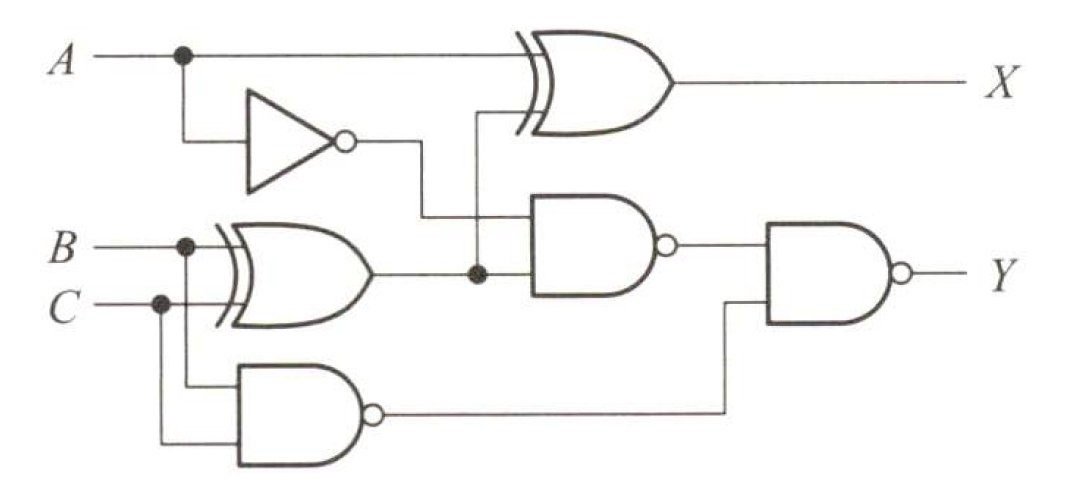
\includegraphics[scale=0.2]{SD4.1.5}
	\caption{4.1.5}
\end{figure}
解:\\

\textbf{Step 1.} 列写逻辑表达式:
$$\begin{aligned}
	X&=A\oplus(B\oplus C)\\
	Y&=\overline{\overline{\overline{A}B\oplus C}\cdot\overline{BC}}\\
	&=\overline{A}(B\overline{C}+\overline{B}C)+BC\\
	&=\overline{A}B+\overline{A}C+BC
\end{aligned}
$$

\textbf{Step 2.} 列写真值表:
\begin{figure}[H]
	\centering
	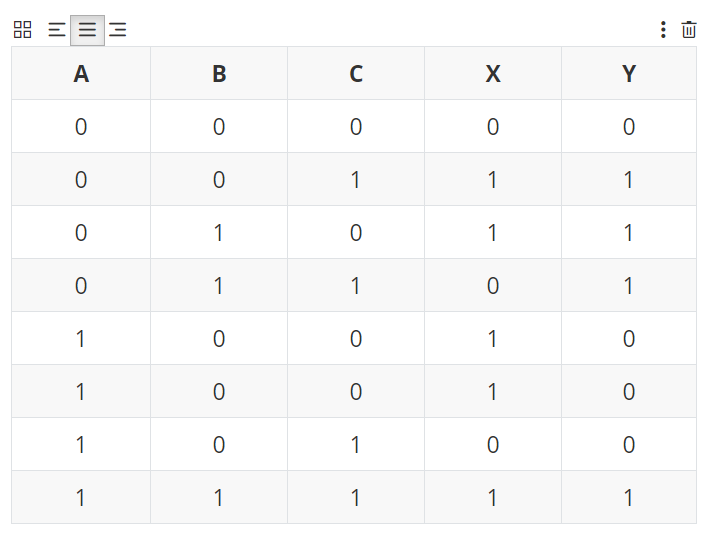
\includegraphics[scale=0.5]{SD4.1.5_1}
	\caption{4.1.5真值表}
\end{figure}
\textbf{Step 3.} 功能分析:

分析不出来。。。\\

\textbf{4.1.6} 分析图题4.1.6所示逻辑电路的功能\\
\begin{figure}[H]
	\centering
	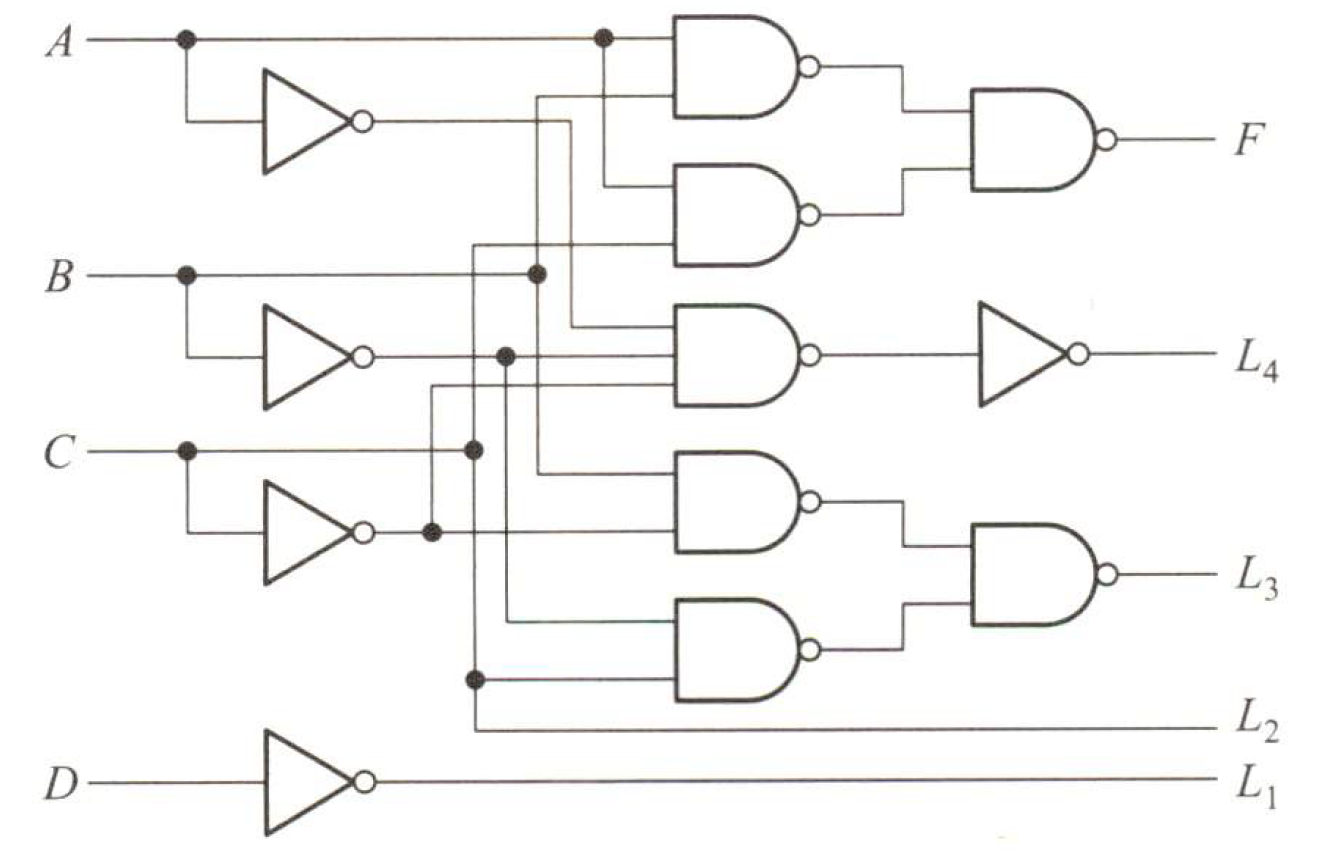
\includegraphics[scale=0.15]{SD4.1.6}
	\caption{4.1.6}
\end{figure}
\noindent 解:\\

\textbf{Step 1.} 列写逻辑表达式:
$$\begin{aligned}
	F&=\overline{\overline{AB}\cdot\overline{AC}}\\
	&=AB+AC\\
	L_4&=\overline{\overline{\overline{A}\cdot\overline{B}\cdot\overline{C}}}\\&=\overline{A}\cdot\overline{B}\cdot\overline{C}\\
	L_3&=\overline{\overline{B\overline{C}}\cdot\overline{\overline{B}C}}\\
	&=B\overline{C}+\overline{B}C\\
	L_2&=C\\
	L_1&=\overline{D}\\
\end{aligned}
$$

\textbf{Step 2.} 列写真值表:
\begin{figure}[H]
	\centering
	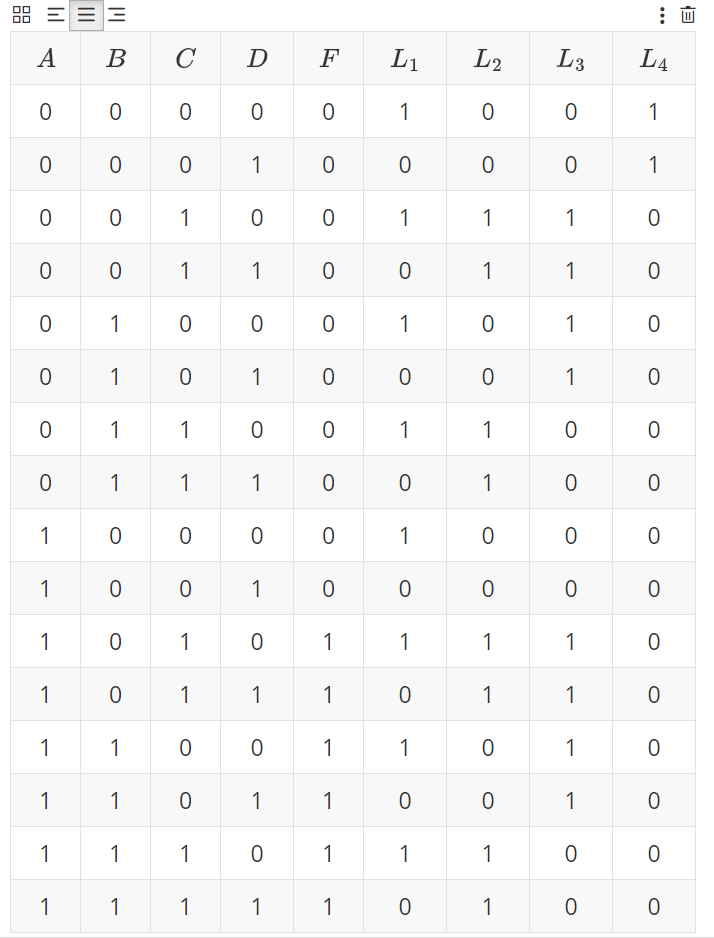
\includegraphics[scale=0.29]{SD4.1.6_1}
	\caption{4.1.6真值表}
\end{figure}
\textbf{Step 3.} 功能分析:
 
注意到$F=0,L_4L_3L_2L_1=9-ABCD,F=1,$ 无意义

\textbf{4.2.9} 某足球评委会由一位教练和三位球迷组成,对裁判员的判罚进行比爱绝。当满足一下条件时表示同意:有三人或三人以上同意,或者两人同意,但其中有一人是教练。试用2输入\textbf{与非}门设计该表决电路(写出完整的设计流程,以及Verilog HDL程序)\\
解:

\textbf{Step 1.} 明确逻辑功能:

设一位教练和和三位球迷分别为$A,B,C,D$, 这些变量为1时表示同意,为0时表示不同意。设输出为L,L=1表示同意判罚,L=0表示否决判罚,则卡诺图(真值表)如下(其中列为AB, 行为CD):
\begin{figure}[H]
	\centering
	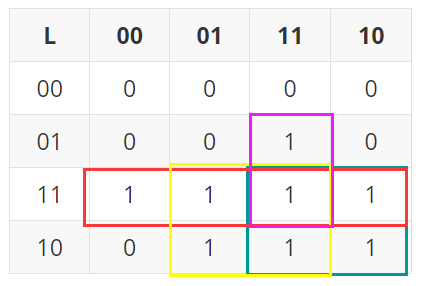
\includegraphics[scale=0.29]{SD4.2.9_1}
	\caption{4.2.9卡诺图}
\end{figure}
\textbf{Step 2.} 列逻辑表达式:

由卡诺图可知:
$$\begin{aligned}
	L&=AB+AC+AD+BCD\\
	&=\overline{\overline{AB}\cdot\overline{AC}\cdot\overline{AD}\cdot\overline{BCD}}\\
	&F=\overline{\overline{\overline{\overline{AB}\cdot\overline{AC}}}\cdot\overline{\overline{\overline{AD}\cdot\overline{\overline{B}\cdot\overline{\overline{CD}}}}}}
\end{aligned}
$$

逻辑电路如下:
\begin{figure}[H]
	\centering
	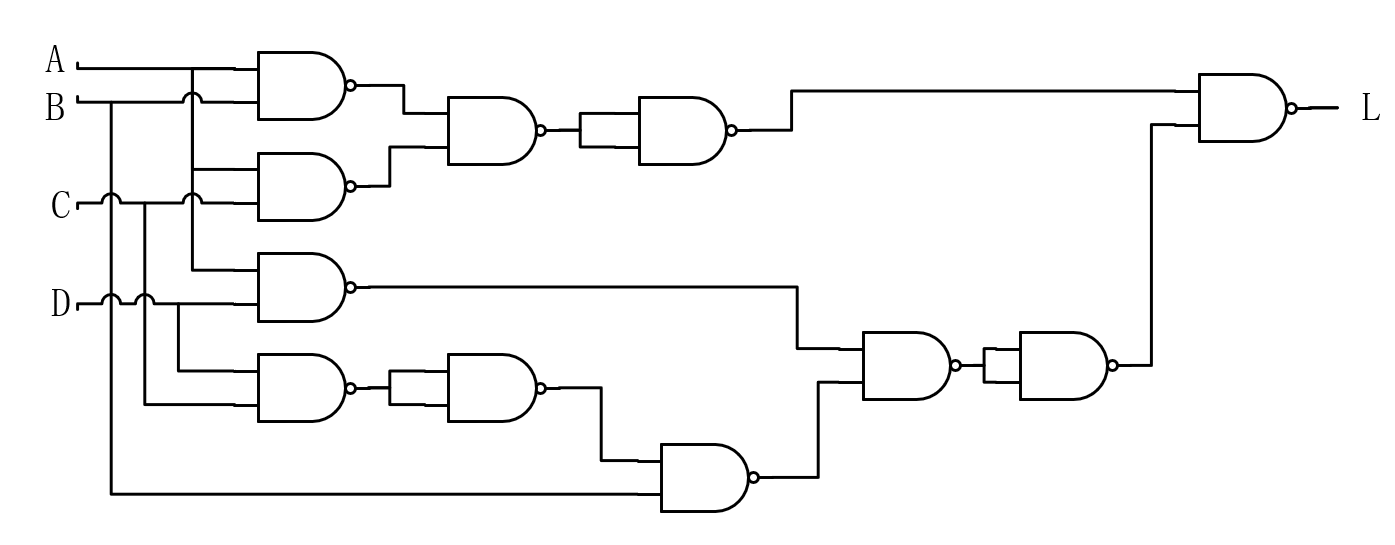
\includegraphics[scale=0.25]{SD4.2.9_2}
	\caption{4.2.9逻辑电路图}
\end{figure}
Verilog HDL语句如下:
\begin{figure}[H]
	\centering
	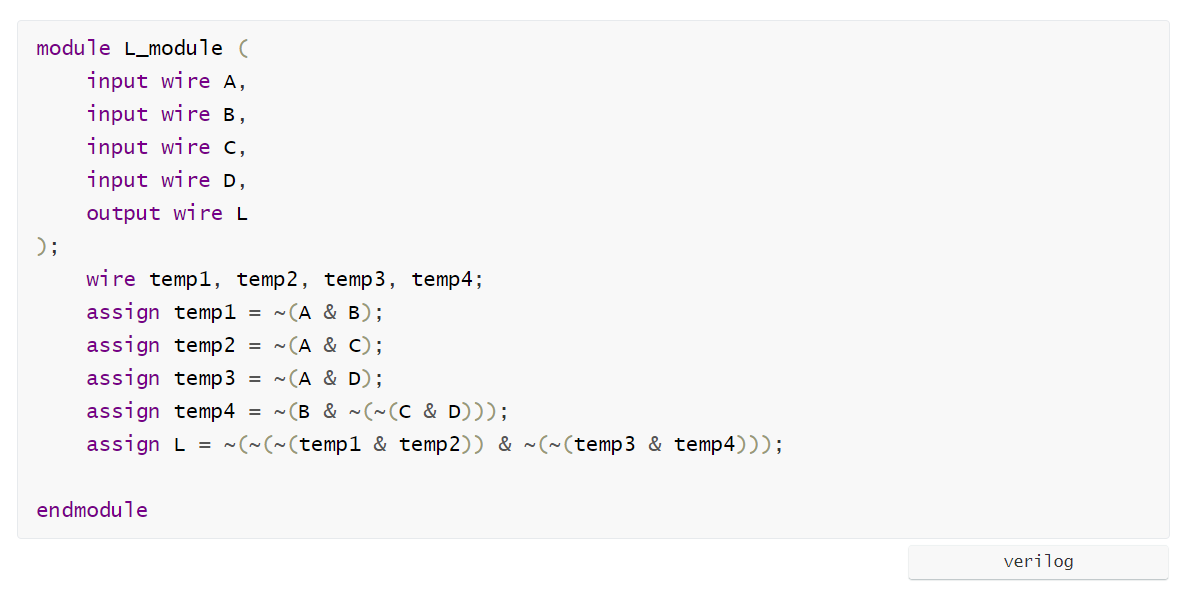
\includegraphics[scale=0.35]{SD4.2.9_3}
	\caption{4.2.9Verilog HDL}
\end{figure}
\textbf{4.2.11} 某火车站有特快、直快和慢车三种类型的客运列车进出,试用2输入与非门和反相器设计一个指示列车等待进展的逻辑电路,3个指示灯一、二、三号分别对应特快、直快、慢车。列车的优先级别依次为特快、直快、慢车,要求当特快列车请求进站时无论其他两种列车是否请求进站,一号灯亮。当特快没有请求,直快请求进站时,无论慢车是否请求,二号灯亮,当特快和直快均没有请求,而慢车有请求时,三号灯亮。(写出完整的设计流程,以及Verilog HDL程序)\\
解:

\textbf{Step 1.} 明确逻辑功能:

设特快、直快、慢车分别为$A,B,C$,当它们取值为1时表示进站,取值为0表示无进站需求,设$L_1,L_2,L_3$分别为一、二、三号灯,取1时灯亮,取0时灯灭。

\textbf{Step 2.} 列逻辑表达式:
$$\begin{aligned}
	L_1&=A\\
	L_2&=\overline{A}B=\overline{\overline{\overline{A}B}}\\
	L_3&=\overline{A}\cdot\overline{B}C=\overline{\overline{\overline{\overline{\overline{A}\cdot\overline{B}}}\cdot C}}\\
\end{aligned}
$$

逻辑电路如下:
\begin{figure}[H]
	\centering
	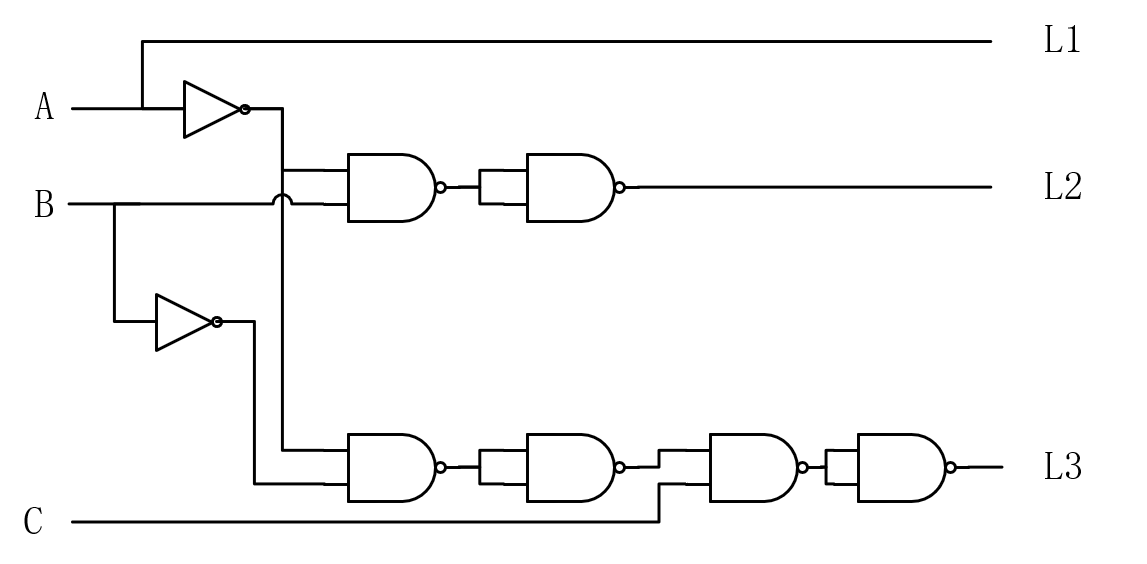
\includegraphics[scale=0.25]{SD4.2.11_1}
	\caption{4.2.11逻辑电路图}
\end{figure}
Verilog HDL语句如下:
\begin{figure}[H]
	\centering
	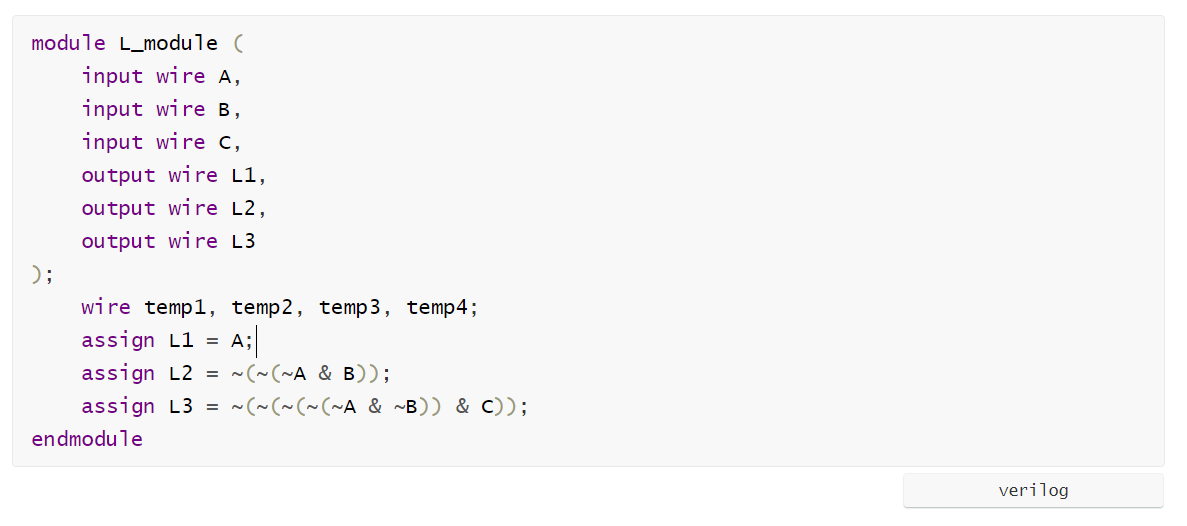
\includegraphics[scale=0.35]{SD4.2.11_2}
	\caption{4.2.11Verilog HDL}
\end{figure}
\textbf{4.2.12} 会议室顶灯分别有安装在4扇门旁边的4个开关控制,设计一个控制电路,要求改变任意一个开关的状态都能打开或关闭顶灯,可以采用任何门电路来实现(写出完整的设计流程,以及Verilog HDL程序)\\
解:

\textbf{Step 1.} 明确逻辑功能:

设这四个开关分别为$A,B,C,D$,取值为1时表示闭合,取值为0表示断开,L为灯,取1表示灯亮,取0表示灯灭,卡诺图(真值表)如下(其中列为AB, 行为CD):
\begin{figure}[H]
	\centering
	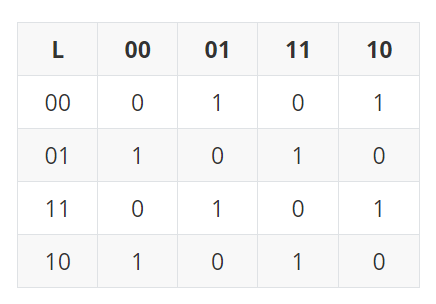
\includegraphics[scale=0.29]{SD4.2.12_1}
	\caption{4.2.12卡诺图}
\end{figure}
\textbf{Step 2.} 列逻辑表达式

由卡诺图可知输出为$A,B,C,D$的异或:
$$\begin{aligned}
	L=A\oplus B\oplus C\oplus D
\end{aligned}
$$

逻辑电路如下:
\begin{figure}[H]
	\centering
	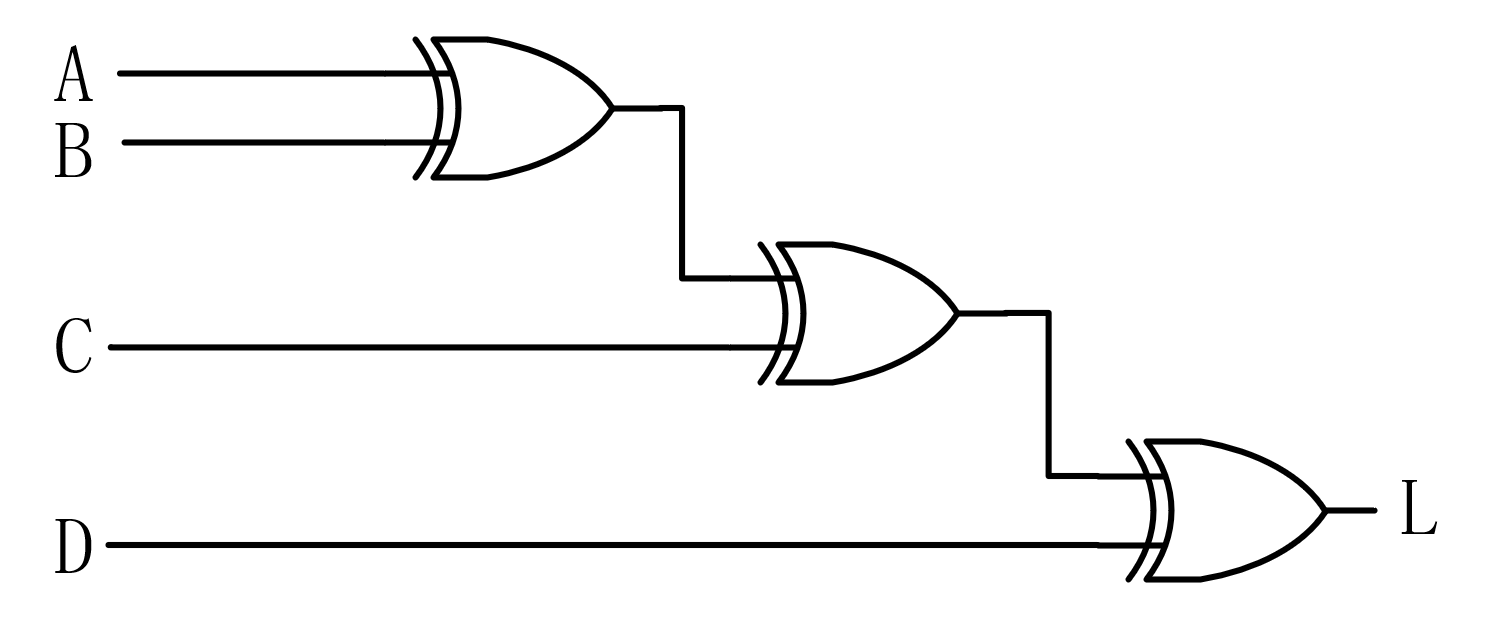
\includegraphics[scale=0.15]{SD4.2.12_2}
	\caption{4.2.12逻辑电路图}
\end{figure}
Verilog HDL语句如下:
\begin{figure}[H]
	\centering
	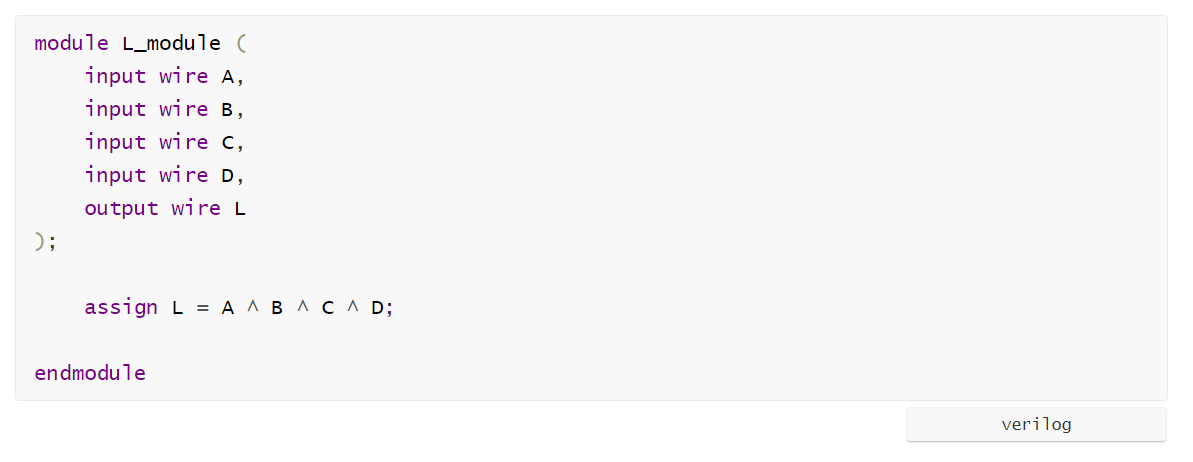
\includegraphics[scale=0.35]{SD4.2.12_3}
	\caption{4.2.12Verilog HDL}
\end{figure}
\textbf{4.2.13} 某化工厂有5种原料,编号为1到5,在使用时必须遵守以下规则:

(1)用第3号时必须使用第1号。

(2)第2号和第4号必须同时使用。

(3)第2号和第5号不能同时使用。

试设计一个逻辑电路,能在违反上述任何一项规定时给出高电平指示信号。写出逻辑表达式。(直接写出表达式并化简,无需Verilog HDL)\\
解:

\textbf{Step 1.} 明确逻辑功能:

设这五种原料分别为$A,B,C,D,E$,取1时为使用,取0时为不使用。设$L$为高电平只是信号,取值为1时为有高电平信号,取0时为无高电平信号。


\textbf{Step 2.} 列逻辑表达式
$$\begin{aligned}
	L=\overline{A}C+B\overline{D}+\overline{B}D+BE
\end{aligned}
$$

画逻辑电路:
\begin{figure}[H]
	\centering
	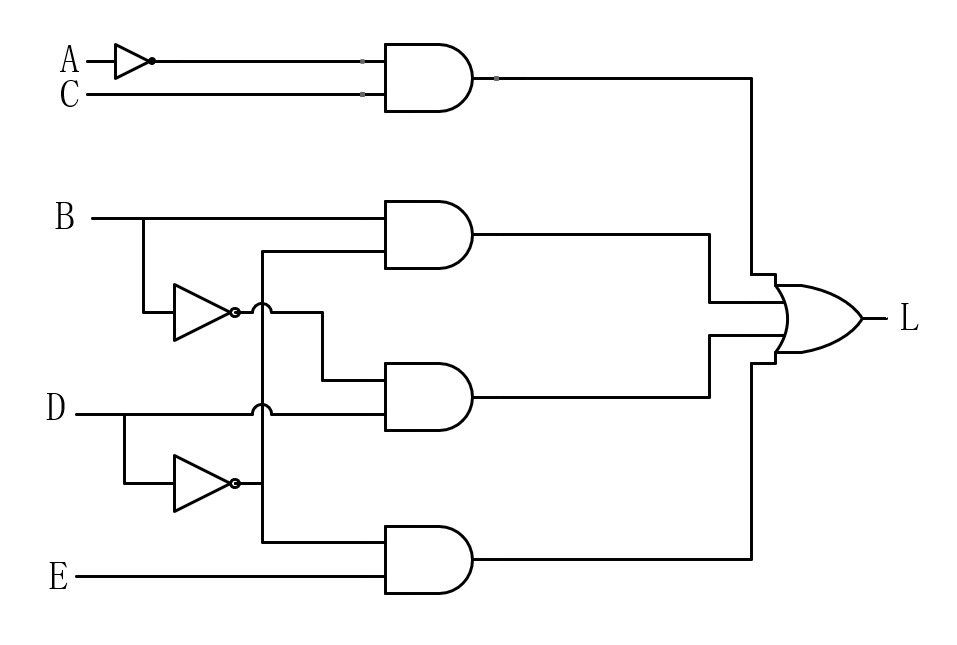
\includegraphics[scale=0.25]{SD4.2.13}
	\caption{4.2.13逻辑电路}
\end{figure}
\textbf{4.2.15} 设计一2为二进制数相加的逻辑电路,可以用任何门电路实现,化简变换时考虑多输出函数的公共乘积项,以减少门的数目。(写出完整设计流程,无需Verilog HDL)\\
提示:
\begin{figure}[H]
	\centering
	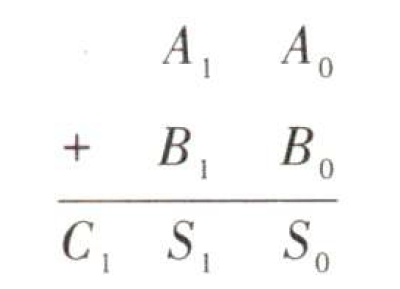
\includegraphics[scale=0.30]{SD4.2.15}
\end{figure}
$A_1,A_0$和$B_1,B_0$分别为的被加数和加数。$S_1,S_0$为相加的和,$C_1$为进位位。\\
解:\textbf{Step 1.} 提示已经给出逻辑功能,我们直接列写真值表:
\begin{figure}[H]
	\centering
	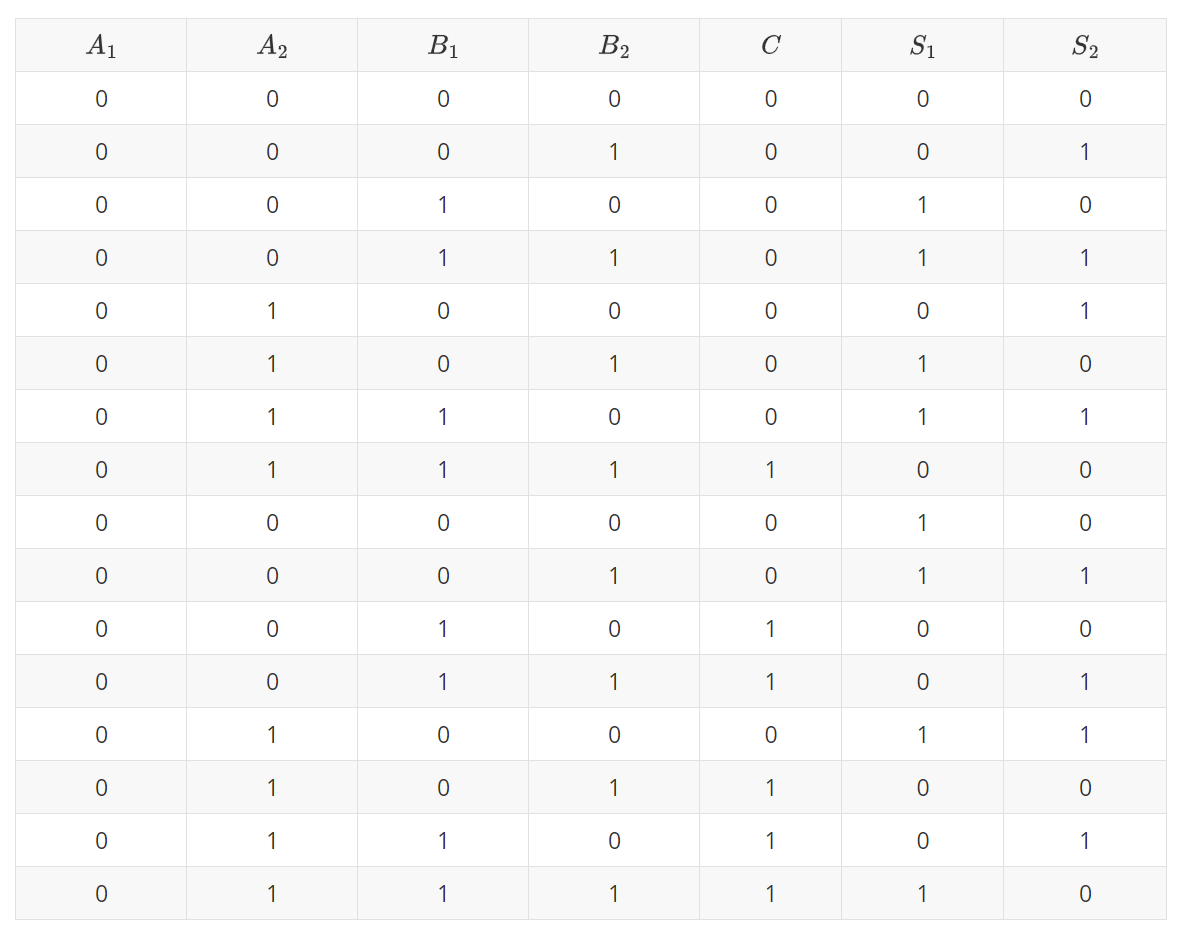
\includegraphics[scale=0.30]{SD4.2.15_1}
	\caption{4.2.15真值表}
\end{figure}
画出卡诺图(其中列为$A_1A_0$, 行为$B_1B_0$):
\begin{figure}[H]
	\centering  %图片全局居中
	\subfigure[$C_1$卡诺图]{
		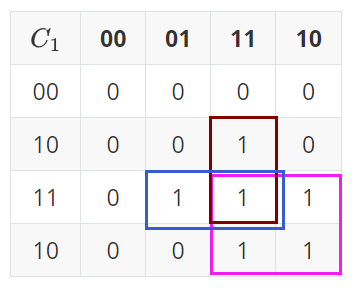
\includegraphics[scale=0.33]{SD4.2.15_2}}
	\subfigure[$S_1$卡诺图]{
		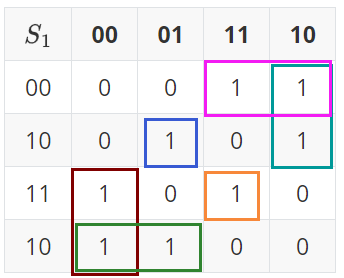
\includegraphics[scale=0.33]{SD4.2.15_3}}
	\subfigure[$S_0$卡诺图]{
		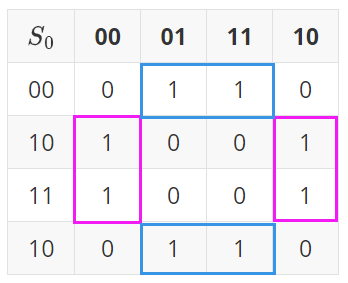
\includegraphics[scale=0.33]{SD4.2.15_4}}
	\caption{4.2.15卡诺图}
\end{figure}
\textbf{Step 2.}列逻辑表达式:
$$\begin{aligned}
	C_1&=A_1B_1+A_1A_0B_0+A_0B_1B_0\\
	S_1&=\overline{A}_1\cdot\overline{A}_0B+\overline{A}_1B_1\overline{B}_0+A_1\overline{A}_0\cdot\overline{B}_1+A_1\overline{B}_1\cdot\overline{B}_0+\overline{A}_1A_0\overline{B}_1B_0+A_1A_0B_1B_0\\
	&=\overline{A}_0(\overline{A}_1B+A_1\overline{B})+\overline{B}_0(\overline{A}_1B_1+A_1\overline{B}_1)+A_0B_0(\overline{A}_1\overline{B}_1+{A}_1{B}_1)\\
	&=A_1\oplus B_1(\overline{A}_0+\overline{B}_0)+A_0B_0(\overline{A_1\oplus B_1})\\
	&=(A_0B_0)\oplus A_1\oplus B_1\\
	S_0&=\overline{A}_0B_0+A_0\overline{B}_0\\
	&=A_0\oplus B_0
\end{aligned}
$$

\textbf{Step 3.} 画逻辑电路:
\begin{figure}[H]
	\centering
	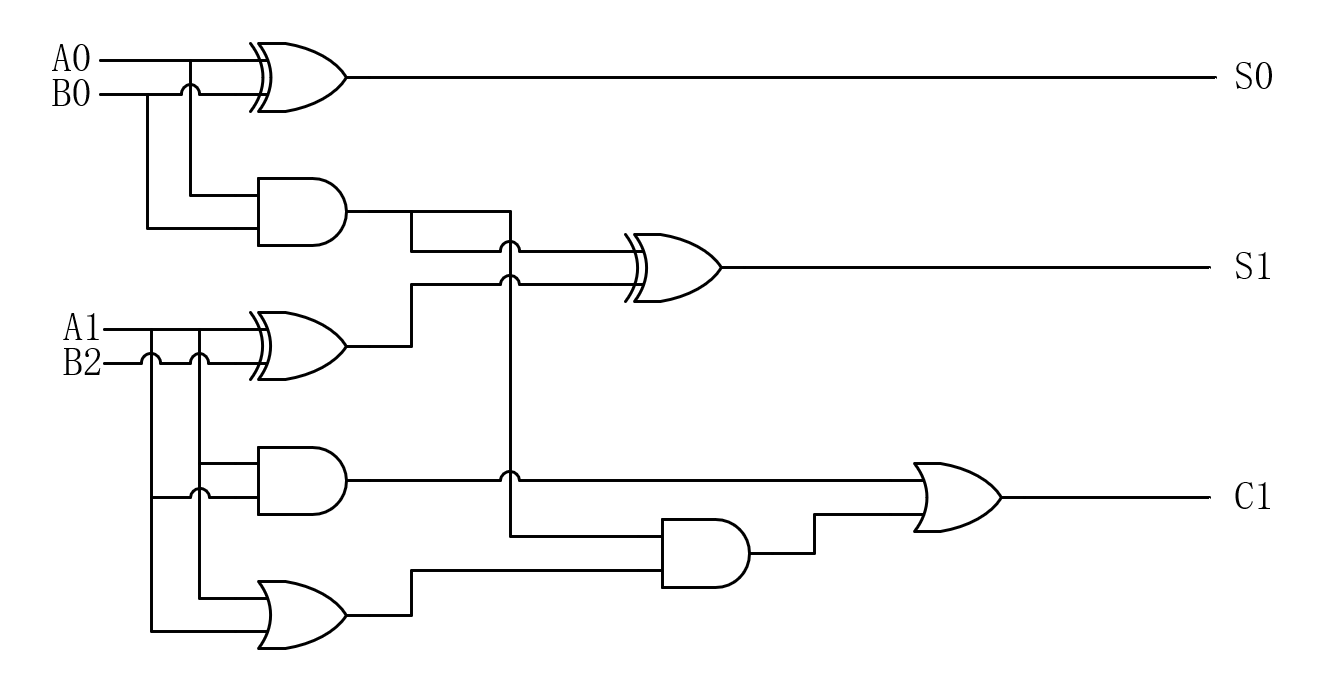
\includegraphics[scale=0.30]{SD4.2.15_5}
	\caption{4.2.15逻辑电路图}
\end{figure}
\end{document}